\documentclass[12pt]{article}

\usepackage{amsmath}

\usepackage{graphicx}



\usepackage[utf8]{inputenc}


\usepackage[spanish]{babel} %Paquete de idioma
\usepackage[hidelinks]{hyperref}
\usepackage{graphicx}
\usepackage{float}

\graphicspath{{images2/}}

\title{Memoria Práctica 1 \\


\large Comunicaciones
}
\author{
Leopoldo Cadavid Piñero
}
\date{Febrero 2022}







\begin{document}

\maketitle
\tableofcontents
\section{Introducción}

      En la siguiente memoria se procederá a explicar las pruebas y resultados obtenidos tras probar el uso de 
      las APIS vistas en clase.\\

      Primero veremos los ejemplos básicos dados en clase para el uso de estas APIS y programas para el manejo de estas:

      \begin{itemize}
        \item \verb|Openweather| 
        \item \verb|REData | 
        \item \verb|Google Colab| 
        \item \verb|Node Red| 
        
    
        
    
        
    \end{itemize}

      Posteriormente veremos en otro apartado la ampliación elegida en la práctica, en la cual se ha 
      trabajado con la API de la app telegram para crear un bot que se conecte con Node red para obtener información de distintas APIS y proporcionarla
      al usuario con a través de distintos comandos.
      

\section{Ejemplo básicos}

\subsection{Openweather}

Lo primero que hemos hecho con Openweather, tras crear una cuenta y obtener nuestra API key, es crear un link  con nuestro id y la 
ciudad de la cual queremos obtener la información.\\

\begin{verbatim}
    http://api.openweathermap.org/data/2.5/weather?q=Alicante,
    ES&mode=json&units=metric&APPID=339f553dbde09f5130892ce20de1dccf
\end{verbatim}
    
Si introducimos el link en el navegador veremos el archivo JSON  de esta manera:    


\begin{figure}[H]
    \centering
    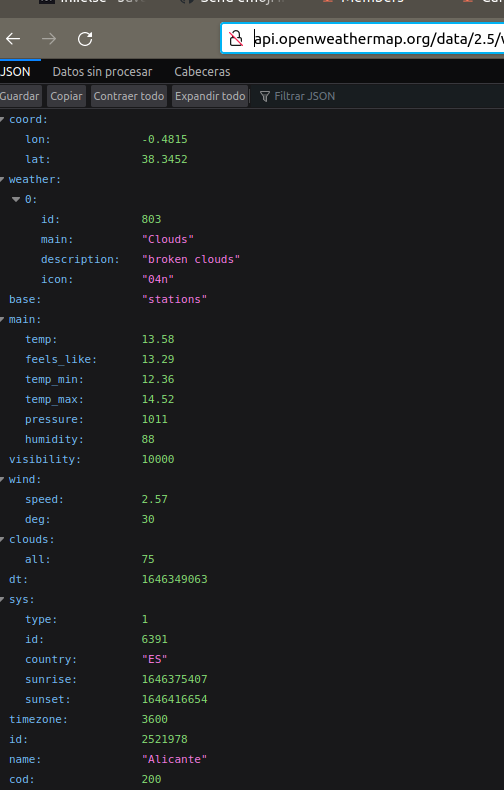
\includegraphics[scale=0.5]{alicantenav.png}
    \caption{Archivo JSON de la API en el navegador}
    \label{fig: alicantenav}
\end{figure}

Una forma de tratar el archivo para tener la información de una forma más limpia sería
utilizando un código de python para para tratar el JSON. Esto lo podemos hacer desde la herramienta Google Colab:

\begin{figure}[H]
    \centering
    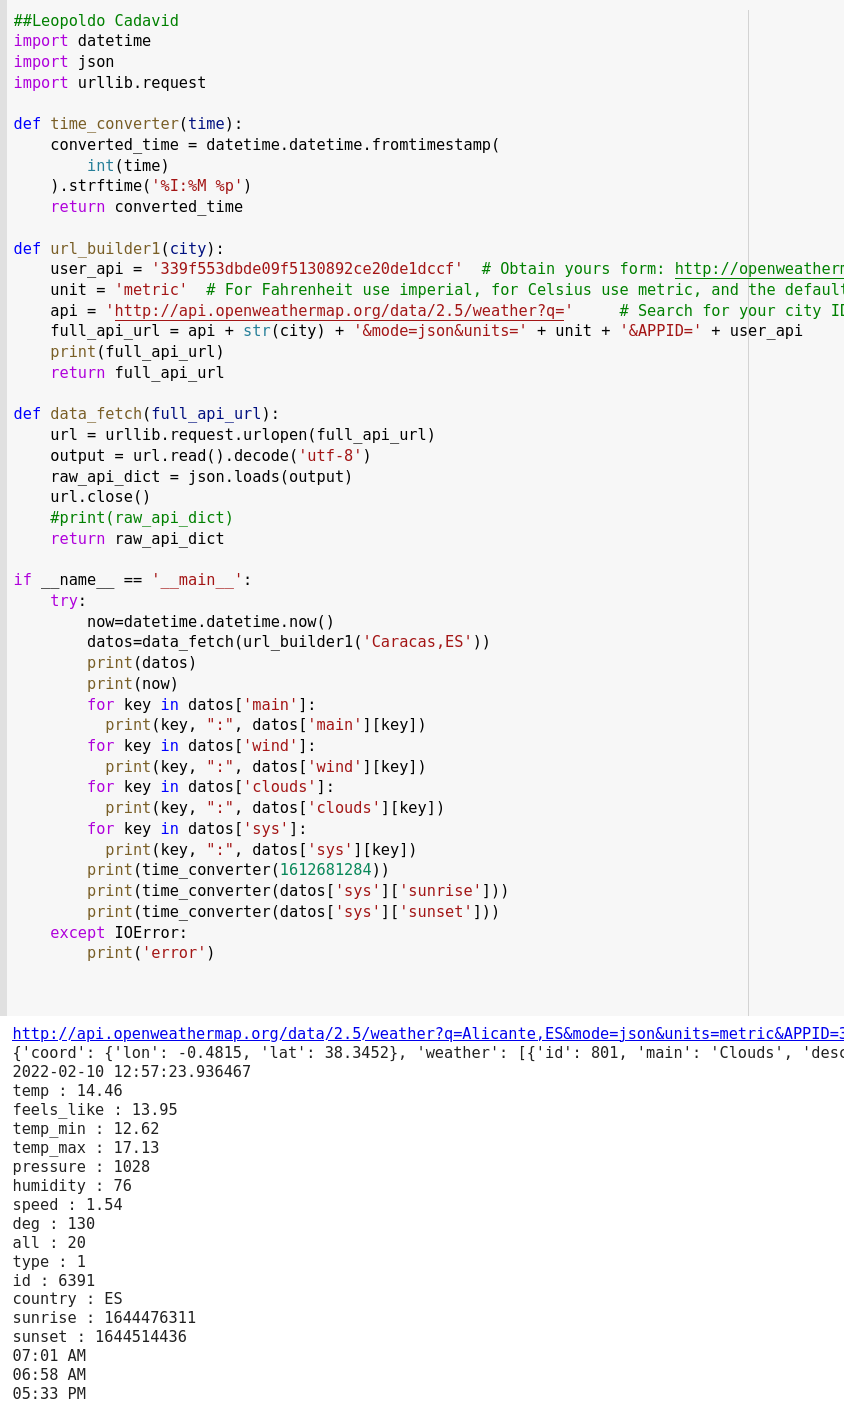
\includegraphics[scale=0.3]{aliopencol.png}
    \caption{Código python y salida desde Colab}
    \label{fig: alicantecolab}
\end{figure}

La siguiente forma de tratar los datos de la api de Openweather es mediante la ampliación \verb|Node Red|. Esta ampliación es 
muy usada en el ámbito de las conexiones entre dispositivos, páginas, etc, ya que mediante una interfaz sencilla e inttuitiva podemos conseguir
conectar y tratar información de distintas apis y combinar estas.\\

En la siguiente imagen veremos el flow hecho para obtener el archivo JSON de Openweather mediante el nodo especifico de Openweather para Node Red.

\begin{figure}[H]
    \centering
    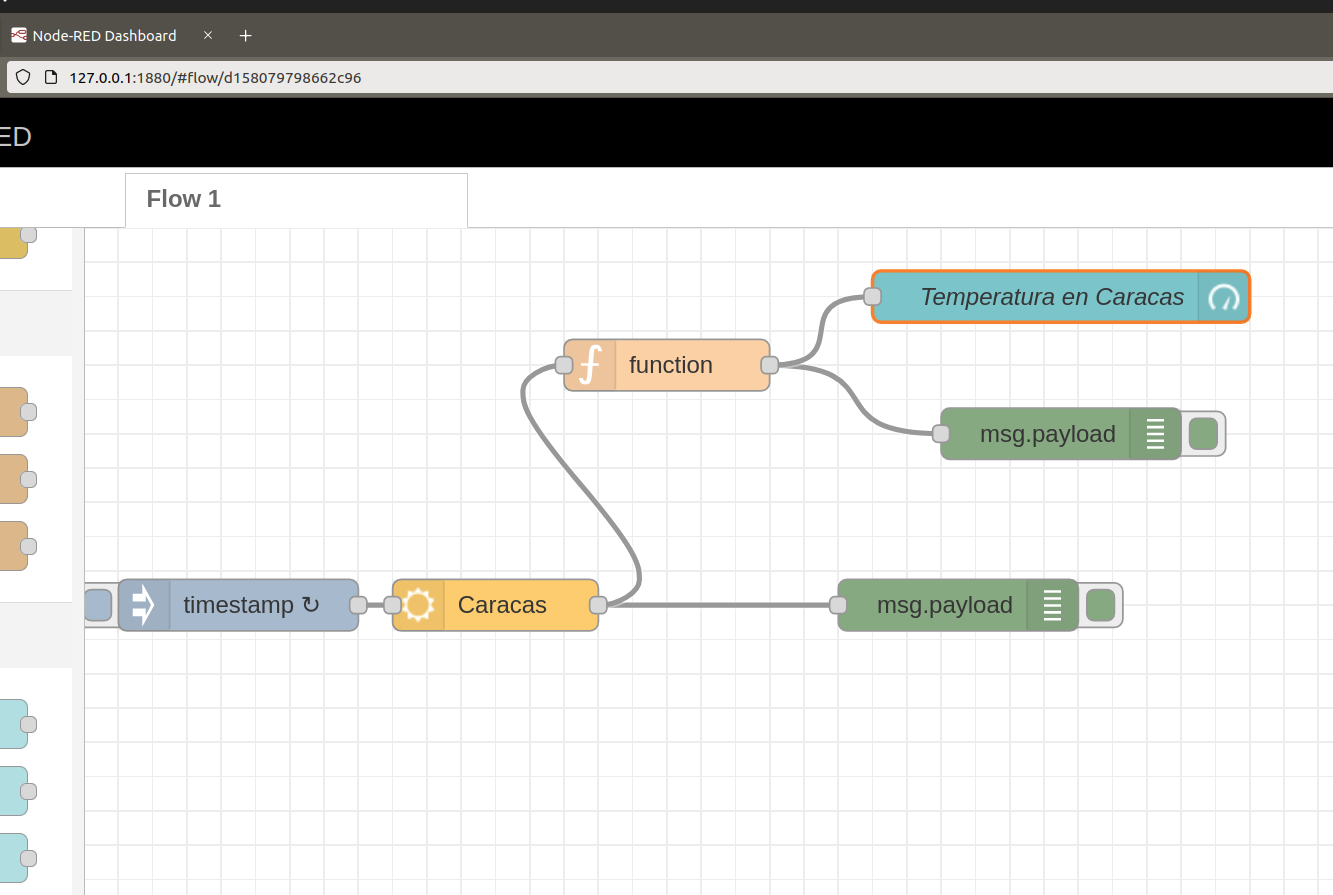
\includegraphics[scale=0.25]{flowcaracas.png}
    \caption{Flow de nodered para obtener la temperatura en Caracas}
    \label{fig: noderedOpenweather}
\end{figure}

El siguiente código sería el que usamos para obtener el contenido de json y lo metemos pasamos al nodo Gauge:
\begin{verbatim}
variable = msg.payload
msg.payload = variable.tempc
return msg;
\end{verbatim}

Y cuando accedemos a la UI  de nodered observamos el resultado:

\begin{figure}[H]
    \centering
    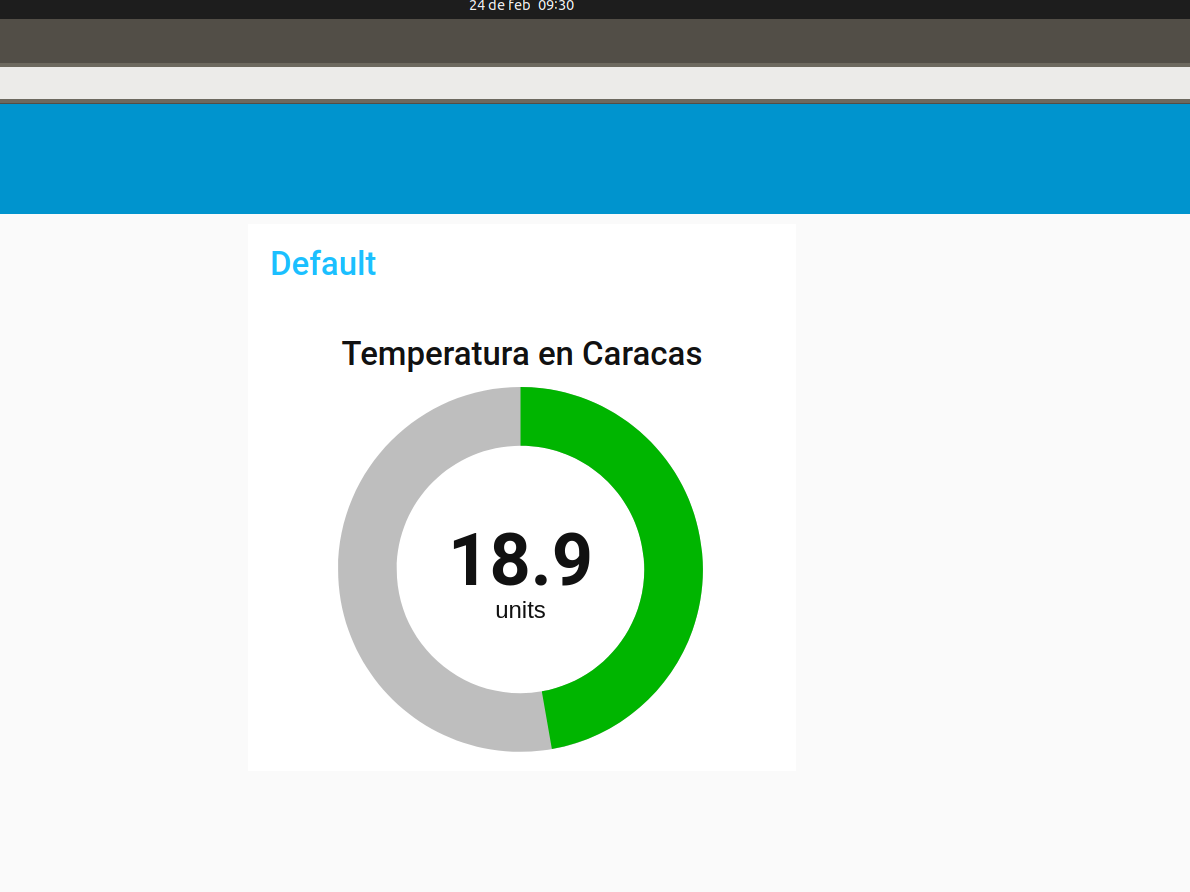
\includegraphics[scale=0.25]{gauge_donut.png}
    \caption{Gauge en formato donut}
    \label{GaugeCaracas}
\end{figure}

\subsection{REData}

La otra api que hemos usado en clase ha sido la del servicio REData, la cual proporciona 
información relacionada con la red electrica española. En ella podemos obtener información de diversos 
ámbitos (mercado, balances, importaciones...). En el siguiente ejemplo vemos una  implementación en nodered, usando el bloque httpRequest
para sacar los archivos JSON. \\

\begin{figure}[H]
    \centering
    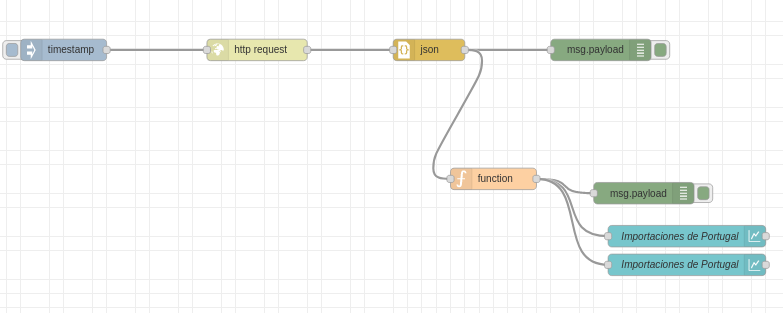
\includegraphics[scale=0.4]{noderedportugal.png}
    \caption{Flow de uso de REData}
    \label{nodeport}
\end{figure}

Y aquí podemos ver la salida en la interfaz de la dashboard.


\begin{figure}[H]
    \centering
    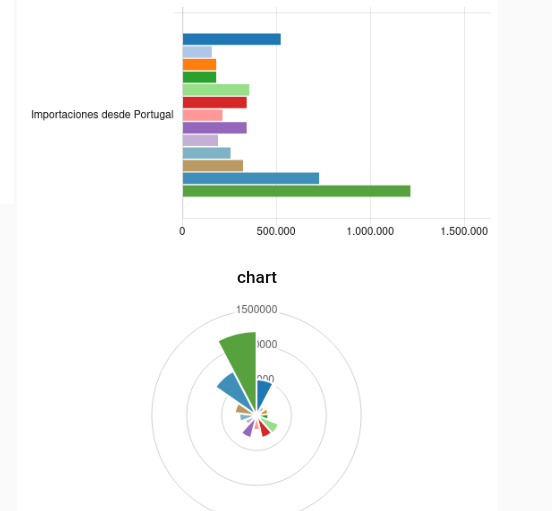
\includegraphics[scale=0.4]{graficasportugal.png}
    \caption{Charts de las importaciones de energía desde Portugal en 2019 por meses}
    \label{grafport}
\end{figure}

\section{Ampliaciones}

La ampliación realizada para la práctica consiste en un bot de telegram que reune todas las APIS vistas y además hace uso de otras nuevas, como la de Telegram, 
manejandolo todo desde Node Red. \\

\subsection{/info}

Este comando proporciona un mensaje con información sobre el bot. Hace uso de
los bloques receiver y sender de la api de telegram
en nodered.

\subsection{/tiempo\_hoy}

\subsection{/caracas}

\subsection{/tiempo\_prediccion}

\section{Link al Github}
Como se comentó en clase, se ha ido actualizando un repositorio de Github con las capturas JSON y códigos usados en la práctica para tener bien documentado todo en caso de que el profesor
requiera consultarlo para la evaluacion de la práctica. el link al repositorio es el siguiente:\\

\verb|https://github.com/leocadpin/Comunicaciones_Leopoldo_Cadavid|



\end{document}